\subsection{Creating The PCB Layout:}

For acid etching, we needed to draw the circuitry using an etchant resistant material. Special markers can be found easily for this specific purpose if we intend to do the drawing by hand (not appropriate for medium to large circuits). But laser printers' ink is the most commonly used material however. This is usually done by converting our circuit's schematic diagram into a PCB layout using PCB layout software. There are many open source software packages for PCB layout creation and design like {\itshape Proteus} or {\itshape Multisim} or {\itshape Liquid PCB}. In Figure 3.1.0 we can find the layout that we are going to work with. \hfill \break

\begin{figure}[H]
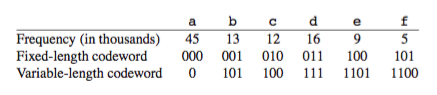
\includegraphics[height = 6cm, width = 16.5cm]{1.png}
\centering \linebreak \linebreak {\small Figure 3.1.0: PCB Layout.}
\end{figure}